\section{Study Selection}
\label{rel-work:study-selection}

\subsection{Start Set}
\label{rel-work-ss:start-set}

My start set is composed of a single paper entitled “How equity and inequity can emerge in pair programming” \cite{lewis:2015}. This paper was cited in an important review in the Cambridge Handbook of Computing Education Research \cite{lewis:2019} and pointed out the gaps and challenges in equity and diversity. This review points to the challenge of considering equity issues and active learning in \gls{CSE}.

\subsection{Inclusion and Exclusion Criteria}
\label{rel-work-ss:inc-exc-criteria}

I used a single inclusion criterion \gls{IC} that was “The work attends to \gls{SRQ}”. In this systematic mapping, all the exclusion criteria served as common reasons to justify the paper exclusion. The \gls{EC} are listed as follows.
\begin{itemize}
    \item The work does not approach Computing Education (\gls{EC}1);
    \item The work does not approach equity (\gls{EC}2);
    \item The work does not approach active methodology (\gls{EC}3);
    \item The work approaches \gls{CEd}, equity, and/or active methodology but does not interlink (\gls{EC}4); and
    \item The work does not fit in the range from 2020 to 2024 (\gls{EC}5).
\end{itemize}

My strategy used each \gls{RC} as follows: (i) title and abstract (\gls{RC}1); (ii) work scanning (\gls{RC}2); and full reading (\gls{RC}3). When \gls{RC}1 failed to exclude the paper, it followed \gls{RC}2. If both criteria were passed, this paper became a real candidate, and we performed \gls{RC}3. 

\subsection{First Iterations}
\label{rel-work-ss:first-iterations}

I conducted two iterations of the snowballing strategy with the specifications described before. I will detail this in the next sections.

\subsubsection{Iteration 0}

This iteration did not backward any paper because the single work in this current start set \cite{lewis:2015} is dated 2015, being all references before 2020 (falling into \gls{EC}5). However, the forward process returned eleven papers after applying \gls{EC} filtering. The search engine used for the generation of the citation list was the Scopus Base, retrieving the last results on July 19, 2024. Figure \ref{fig:first-iteration} presents the diagram of the whole iteration.

\begin{figure}[htb]
\centering

\caption{\textmd{Diagram of Iteration 0 after snowballing strategy.}}
\label{fig:first-iteration}
\fcolorbox{gray}{white}{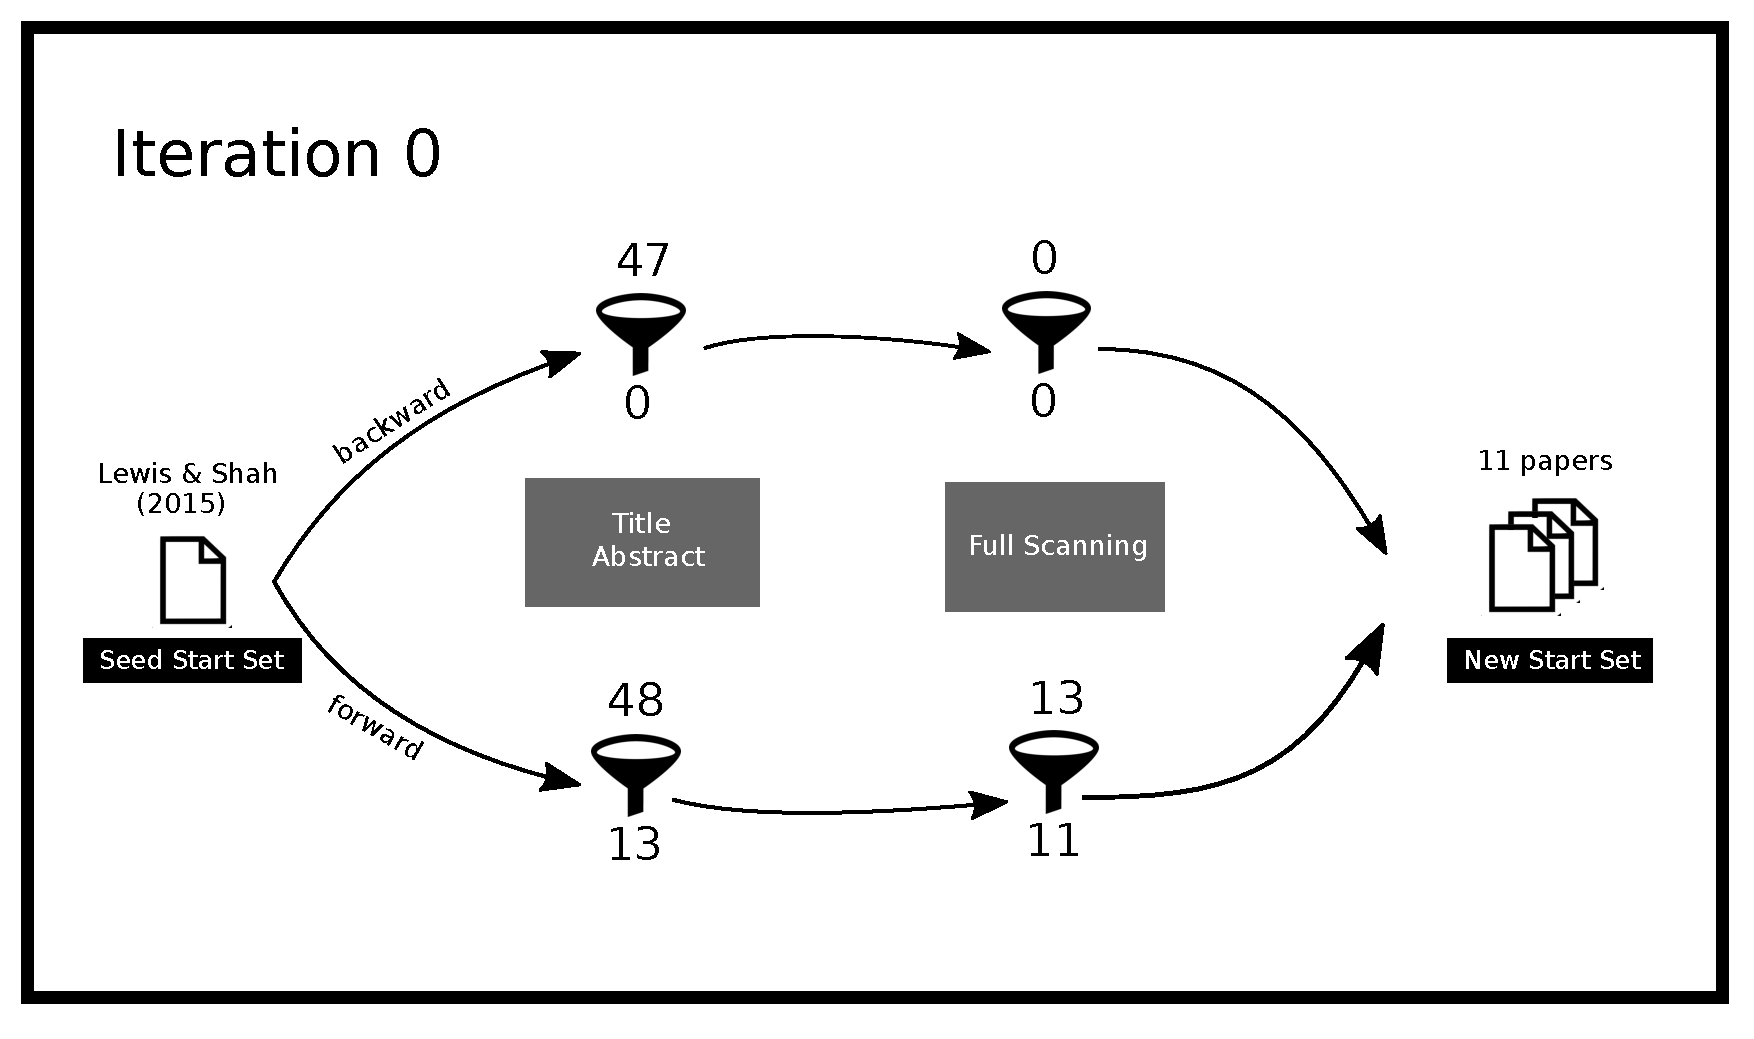
\includegraphics[width=0.95\textwidth]{images/chapter-04/first-iteration.pdf}}

\par\medskip\ABNTEXfontereduzida\selectfont\textbf{Source:} Created by the author (2024).
\end{figure}

Thus, at the end of this iteration, the paper set increased from one to eleven papers (see Table \ref{tbl:iteration-0-list-papers}), bearing in mind that the work \cite{lewis:2015} was chosen strategically, aiming to capture newer works after 2020 (inclusive).

\begin{table}[htb]
\caption{List of the papers of the new start set identified during the 
Iteration 0 after snowballing strategy.}
\label{tbl:iteration-0-list-papers}
\centering
\rowcolors{1}{}{lightgray}
\begin{tabular}{
    m{7cm}|
    m{7cm}
}
    \hline
    \multicolumn{2}{c}{
        \textbf{Seed Start Set}
    }\\
    \hline
    \multicolumn{2}{c}{
        \citeonline{lewis:2015}
    }\\   
    \hline
    \multicolumn{2}{c}{
        \textbf{New Start Set}
    }\\
    \hline
    \citeonline{arawjo:2021} &
    \citeonline{ayub:2020} \\

    \citeonline{bodaker:2023} &
    \citeonline{grabl:2024} \\
    
    \citeonline{gransbury:2022} &    
    \citeonline{izhikevich:2022} \\
    
    \citeonline{love:2021} &    
    \citeonline{lui:2020} \\
    
    \citeonline{lyttle:2020} &    
    \citeonline{musaeus:2022} \\
    
    \citeonline{ying:2021} &
    \\
    \hline
    
\end{tabular}

  \par\medskip\ABNTEXfontereduzida\selectfont\textbf{Source:} Created by the author (2024). \par\medskip
\end{table}

\subsubsection{Iteration 1}

The backward process of Iteration 1 returned 11 papers after applying \gls{EC} filtering. In the next step, the forward process returned 9 papers after applying \gls{EC} filtering. The search engine used for the generation of the citation list was also the Scopus Base, retrieving the last results on July 22, 2024. Figure \ref{fig:second-iteration} presents the diagram of the whole iteration.

Thus, at the end of this iteration, the paper set increased from 11 to 31 papers (see Table \ref{tbl:iteration-1-list-papers}). I released all detailed information about the study selection in an online public repository\footnote{The snowballing information of this mapping is available on this \gls{Ph.D.} public repository: \url{https://github.com/bispojr/phd-info}.}, structuring through a spreadsheet with all decisions made in this stage.

\begin{figure}[htb]
\centering

\caption{\textmd{Diagram of Iteration 1 after snowballing strategy.}}
\label{fig:second-iteration}
\fcolorbox{gray}{white}{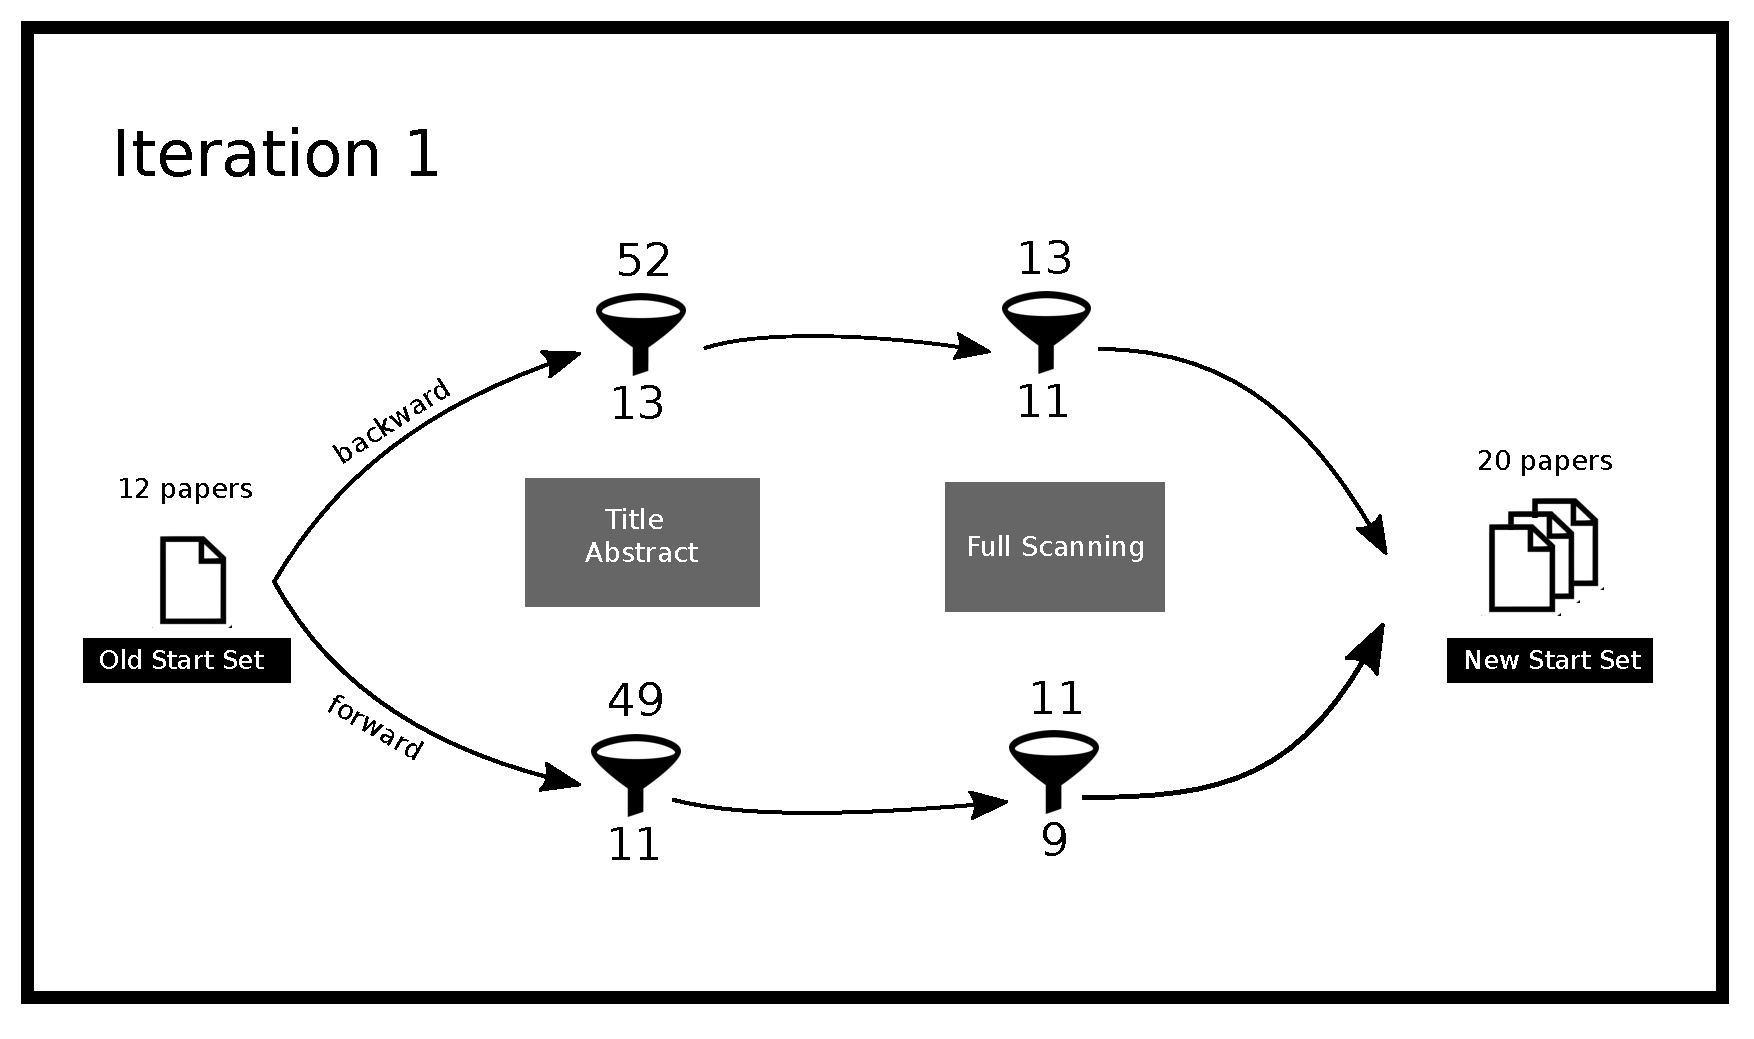
\includegraphics[width=0.95\textwidth]{images/chapter-04/second-iteration.pdf}}

\par\medskip\ABNTEXfontereduzida\selectfont\textbf{Source:} Created by the author (2024).
\end{figure}